% https://apcz.umk.pl/czasopisma/index.php/sztukaedycji/index
% https://apcz.umk.pl/czasopisma/index.php/sztukaedycji/about/submissions#authorGuidelines
% Janusz S. Bień
% Formal Linguistics Department, University of Warsaw, Dobra 55, 00-312 Warszawa, Poland
% jsbien@uw.edu.pl

\documentclass{article}
\usepackage{fontspec}
\usepackage{polyglossia}
\usepackage{etoolbox}
\setmainlanguage{english}
%\setotherlanguage{english}
\usepackage{csquotes}
\usepackage{wrapfig}
\usepackage[style=authoryear,backend=biber,backref=true,urldate=short]{biblatex}
\addbibresource{all.bib}

% http://tex.stackexchange.com/questions/166337/quotation-mark-quotation-sign-xelatex-polyglossia-csquotes
\DeclareQuoteStyle{polish}% I looked it up on Wikipedia, no idea if it's right
  {\quotedblbase}
  {\textquotedblright}
  [0.05em]
  {\textquoteleft}
  {\textquoteright}

% psuje tytuły???:
%  \usepackage{ulem}
\usepackage{metalogo}
\usepackage{varioref}
\usepackage{xcolor}


\def\eob{ę}

% \setmainfont[Mapping=tex-text]{TeX Gyre Termes}
%\setmainfont[Mapping=tex-text]{Lato-Regular}
%\setmainfont[Mapping=tex-text]{GentiumPlus-R}
%\setmainfont[Mapping=tex-text]{LiberationSerif}
\setmainfont[Mapping=tex-text]{JuniusX}
%\setmainfont[Mapping=tex-text]{FreeSerif}
% \char"EC10 \char"EC11 oraz \char"EC12
\def\orogate{\char"EC12}
\def\medievalcomma{{\fontspec{Unifont}⹌}}
\def\Hb#1{{\fontspec{Junicode}#1}}
\def\Htest{{\fontspec{Unifont}M⁹¹}}
% \newcommand{\J}[1]{{\fontspec[Path=/home/jsbien/Junicode/]{Junicode.ttf}#1}}
% \def\Sł{{\fontspec[Path=/home/jsbien/Junicode/]{Junicode.ttf}\char"E8DF}}

\newfontfamily\J[Color=green]{JuniusX}
\newfontfamily\bJ[Color=violet]{Junicode}
%\newcommand{\J}[1]{{\bJ#1}}
\def\Sł{{\fontspec{Junicode.ttf}\char"E8DF}}
% buster: Missing character: There is no  in font [Junicode.ttf]/OT:script=latn;language
\newfontfamily\bS[Color=violet]{Symbola}
\newcommand{\Sy}[1]{{\bS#1}}
\newcommand{\Ju}[1]{{\bJ#1}}

\usepackage{relsize}

\usepackage[breaklinks]{hyperref}

\usepackage{graphicx}
% [hyphens]: options clash
\usepackage{url}
%\usepackage{natbib}

% program name
\newcommand{\pname}[1]{\textsf{#1}}


% file name
\newcommand{\fname}[1]{\texttt{#1}}

\newcommand{\uname}[1]{\texttt{'#1'}}
\newcommand{\ucode}[1]{\texttt{U+#1}}
\newcommand{\usi}[1]{\texttt{#1}}

% Aletheia
\newcommand{\aname}[1]{\texttt{#1}}
\newcommand{\acode}[1]{\texttt{#1}}

% MUFI
\newcommand{\mname}[1]{\texttt{'#1 \textsc{<mufi>'}}}
\newcommand{\mcode}[1]{\texttt{M+#1}}



\usepackage{draftwatermark}
\usepackage[doublespacing]{setspace}

\usepackage{xfrac}

% ni edziała:?
\renewcommand{\topfraction}{0.9}
\renewcommand{\floatpagefraction}{0.9}	% require fuller float pages

\newcommand{\Jglyph}[1]{{\relsize{2}\J#1}}

%\gappto\captionslingua{\renewcommand{\chaptername}{Caput}}
%\gappto\captionspolish{\renewcommand{\figurename}{Ilustracja}}


% \newcommand{\uname}[1]{{\relsize{-1}\texttt{#1}}}
% \newcommand{\ucode}[1]{\texttt{#1}}
% \newcommand{\mname}[1]{\texttt{#1}}
% \newcommand{\mcode}[1]{\texttt{#1}}
% \newcommand{\aname}[1]{\texttt{#1}}
% \newcommand{\acode}[1]{\texttt{#1}}
% \newcommand{\prname}[1]{\textsf{#1}}

%\usepackage[mark]{gitinfo2}

\begin{document}

\title{Usage of Unicode Plane 15 in JuniusX font\\ (a Polish perspective)}
%\title{Textel names proposal for JuniusX\\ Unicode plane 15 characters}

\author{Janusz S. Bień}

%\date{\today\\\gitAuthorIsoDate}
\date{\today}

\maketitle

\catcode`\&=11
\catcode`\|=11
\catcode`\_=11

% The notion of textel was proposed ???

% JuniusX ???

% Unicode

% kenmcd20:_junius_user_guide_first_draft,
% https://unicode.org/mail-arch/unicode-ml/y2017-m03/0031.html

% The notion of textel was proposed by Janusz S. Bień,
% cf. eg. %\cite{bc160} and
% \autocite{bc381}; it was mentioned several times at the Unicode
% mailing list,
% cf. e.g.\url{https://www.unicode.org/mail-arch/unicode-ml/y2016-m09/0040.html}.
% % \url{https://unicode.org/mail-arch/unicode-ml/y2017-m03/0031.html}.

\section{Introduction}
\label{sec:introduction}



JuniusX font (\url{https://psb1558.github.io/Junicode-New/}) is the
succesor to Junicode (\url{https://junicode.sourceforge.io/}), both
fonts has been created by Peter Baker. It is a font featuring in
particular full compliance with the Medieval Unicode Font Initiative
specification (version 4.0) and including all medieval characters
added since MUFI 4.0 (\url{https://mufi.info/}). The font is available
on the principes of the SIL Open Font License (OFL)
v. 1.1\footnote{\url{https://scripts.sil.org/cms/scripts/page.php?site_id=nrsi&id=OFL}}
(SIL International is the successor of the Summer Institute of
  Linguistics for training missionaries).

  The fonts includes also character variants suggested by users, in
  particular several characters needed for old Polish texts and not
  available elsewhere.
  
  Regular Unicode characters have alot of various propertied,
  properties described in the so called Unicode Character
  Database. The properties are used directly or indirectly by
  applications, in particular by OpenType rendering engines.

  MUFI uses Private Use Area characters, but does not provide
  explicitely their properties. There was an attempt to provide them
  in a way mimicking The Unicode Character
  Database\footnote{\url{http://www.kreativekorp.com/charset/PUADATA/PUBLIC/MUFI/}},
  but applications are not capable to make use of such unofficial
  information\footnote{cf. e.g. \url{http://www.unicode.org/mail-arch/unicode-ml/y2018-m08/0095.html}
    and \url{https://debbugs.gnu.org/cgi/bugreport.cgi?bug=32599}}.

  One of the design goals of JuniusX was to supercede PUA characters
  by various features of OpenType
  fonts\footnote{Cf. e.g. \url{https://docs.microsoft.com/en-us/typography/opentype/spec/featurelist}},
  such as
  \begin{itemize}
  \item \texttt{calt} (Contextual Alternates)
  \item \texttt{cv} (Character Variant)
  \end{itemize}
  
  Despite the advantages of such
  approach\footnote{Cf. e.g. \url{https://psb1558.github.io/Junicode-New/Searchability.html}}
  there still some important applications which cannot handle them (at
  least without modification). One of them is \pname{djview4poliqarp}
  (\url{https://bitbucket.org/mrudolf/djview-poliqarp/}), which does
  not support OpenType features, for indexes such as
  \url{https://github.com/jsbien/Zaborowski-index4djview}.

  Using OpenType feature is also of no use for encoding texts to be
  included in linguistic corpora (it's theretically possible to
  translate them into an appropriate markup such as that formulated by
  Text Encoding Initiative, but it makes corpus processing much more
  complicated). For example, in the IMPACT corpus \autocite{bc289} the
  letters \textit{ą} and \textit{ę} and their variants with the stroke
  instead of ogonek occured with almost the same frequency. The stroke
  variants has been represented by {ⱥ} (\uname{2C65}) and {ɇ}
  (\uname{0247}), but this was considered a temporary solution as the
  glyphs differ significally.

  The solution is to duplicate in the Private Use Area the character
  variant accessible with OpenType features. Is the primary Private
  use Area, i.d. \ucode{E000}-\ucode{F8FF} is rather crowded and
  already used for conflicting assignments, the decision was made to
  use plane 15 (\ucode{F0000} – \ucode{FFFFD}). It seems to be the
  very first usage of plane 15.

  One of the important Unicode character property is its name. In the
  present paper names, following the Unicode naming rulse, are
  proposed for private use characters assigned in the font to plane
  15. Additionally the names are provided in the format suitable to
  use it with
  \pname{fntsample-with-comments}\footnote{Cf. \url{https://github.com/psb1558/Junicode-New/discussions/49}}
  to produce a Unicode-like font tables.
 
Some principles of the naming policy are:
\begin{itemize}
\item Comments in brackets are considered as a part of the name by
  \textsf{Unihistext}, but not necessarily in other circumstances.
\item Every proper name ends in VARIANT
\item Names try to follow English Unicode usage. The term
  \textit{terminal} comes from
  \autocite{gaskell76:_nomec_letter_roman_type}.
% \item ; when appropriate, MUFi names are used or adapted. MUFI codes
%   in comments are prefixed with M+.

\end{itemize}

 
 Some characters presented here has been used in critical or didactic
 editions of old Polish manuscripts, such as
 \autocite{vrtel-wierczyński50:_wybór}. It is worth noting that the
 second edition is primarily a photo-offset reproduction of the 1930
 first printing; one of the reasons was the difficulty to find a printing
 house, where the type needed for old Polish survived the WW II.

The best way to access links in the paper to DjVu documents is to use
appropriately configured External Application Button extension
(\url{https://github.com/andy-portmen/external-application-button/issues/50})
available for popular browsers.

\section{List of characters}
\label{sec:list-characters}



\begin{description}
\item[0xF0000] LATIN CAPITAL LETTER A WITH STROKE THROUGH TERMINAL
  VARIANT [JuniusX]: \Jglyph{󰀀}.\\
  Cf. \url{https://github.com/psb1558/Junicode-New/issues/14}.
  % The
  % term \textit{terminal} used after ???.\\
  
  In JuniusX font accessible also as \textit{Ą} with \texttt{cv02[1]};
  % a slightly different glyph available as \texttt{cv02[2]},
  % cf. \autocite[p. 7]{baker20:_opent_featur_junius_junius}.
  cf.  0xF001E  below for a slightly different glyph.

  May be considered also as a variant of LATIN CAPITAL LETTER A WITH
  STROKE (U+023A).

  Occurs in particular in \textit{Nowe Ateny} (1756,
  \url{http://www.wbc.poznan.pl/Content/6625/index.djvu?djvuopts=&page=2186.djvu},
  cf. Fig. \vref{fig:NA1756}.

  \begin{figure}[h]
    
\includegraphics{img/00433085patrzacey}
    \caption{{\J PATZR󰀂CEY} (1756)}
    \label{fig:NA1756}
  \end{figure}

\item [0xF0001] LATIN SMALL LETTER A WITH STROKE THROUGH TERMINAL VARIANT [JuniusX]: 
  \Jglyph{󰀁}.\\ Cf. \url{https://github.com/psb1558/Junicode-New/issues/14};
  % The
  % term \textit{terminal} used after ???.
  cf. 0xF001F below for a slightly different glyph.

  In JuniusX font accessible also as \textit{ą} with \texttt{cv02[1]};
  a slightly different glyph available as \texttt{cv02[2]},
  cf. \autocite[p. 7]{baker20:_opent_featur_junius_junius}.


  May be considered also as a variant of LATIN SMALL LETTER A WITH
  STROKE (U+2C65).

  Occurs in particular in \textit{Nowe Ateny} (1756, \url{
    http://www.wbc.poznan.pl/Content/6625/index.djvu?djvuopts=&page=2355.djvu},
  cf. Fig. \vref{fig:NA1756a}.
 

  \begin{figure}[h]
    
\includegraphics[width=1.3\textwidth]{img/00433254czescZtad.png}
    \caption{{\J części󰀁 [ldots] t󰀁d} (1756)}
    \label{fig:NA1756a}
  \end{figure}


\item [0xF0002] LATIN CAPITAL LETTER A WITH EXTENDED OGONEK VARIANT [JuniusX]: 
  \Jglyph{󰀂}.\\ Cf. \url{https://github.com/psb1558/Junicode-New/issues/14}.
  % The
  % term \textit{terminal} used after ???.

  In JuniusX font accessible also as \textit{Ą} with \texttt{cv02[3]};
  cf. \autocite[p. 7]{baker20:_opent_featur_junius_junius}.

  %   May be considered also as a variant of LATIN CAPITAL LETTER A WITH
  % STROKE (U+023A).

  Occurs at least in \textit{Zbiór rytmów duchownych Panegirycznych
    Moralnych i Swiatowych [...] Elżbiety z Kowalskich Druzbackiey}
  (1752,
  \url{http://www.wbc.poznan.pl/Content/22431/directory.djvu?djvuopts=&page=0242_0001.djvu}.
  cf. Fig. \vref{fig:Rytmy1752}.

  \begin{figure}[h]
    
\includegraphics{img/00487576ksiazecia}
    \caption{{\J XI󰀂ZĘCIA} (1752)}
    \label{fig:Rytmy1752}
  \end{figure}
  
\item [0xF0003] LATIN SMALL LETTER C WITH MEDIUM HIGH OVERLINE VARIANT [JuniusX]: 
  \Jglyph{󰀃}.\\ Cf. \url{https://github.com/psb1558/Junicode-New/discussions/44#discussioncomment-202860}.

    In JuniusX font accessible  with \texttt{ss05};
  cf. \autocite[p. 7]{baker20:_opent_featur_junius_junius}.

  
\item [0xF0004] LATIN SMALL LETTER C WITH HIGH OVERLINE VARIANT [JuniusX]: 
  \Jglyph{󰀄}.\\ Cf. \url{https://github.com/psb1558/Junicode-New/discussions/44#discussioncomment-202860}.

  In JuniusX font accessible  with \texttt{ss04};
  cf. \autocite[p. 6]{baker20:_opent_featur_junius_junius}.

\item [0xF0005] LATIN SMALL LETTER INSULAR D VARIANT [JuniusX]:\\
  \Jglyph{󰀅}.%\\ %Cf. \url{https://github.com/psb1558/Junicode-New/issues/14}.

  In JuniusX font accessible also as \textit{d} with \texttt{cv05[2]};
  cf. \autocite[p. 7]{baker20:_opent_featur_junius_junius}.

  May be considered also as a variant of LATIN SMALL LETTER INSULAR D (U+A77A).
% 

\item [0xF0006] LATIN SMALL LETTER ETH VARIANT [JuniusX]: 
  \Jglyph{󰀆}.\\ Cf. \url{https://github.com/psb1558/Junicode-New/discussions/44#discussioncomment-202860}.

  In JuniusX font accessible also as \textit{ð} (U+00F0) with
  \texttt{ss01} when \texttt{loca} enabled;
  cf. \autocite[p. 11]{baker20:_opent_featur_junius_junius} and
  \autocite[p. 4 (30)]{kenmcd20:_junius_user_guide_first_draft}.
% ð LATIN SMALL LETTER ETH

\item [0xF0007] LATIN SMALL LETTER D WITH STROKE ROUNDED VARIANT [JuniusX]:\\
  \Jglyph{󰀇}.\\
  Cf. \url{https://latin.stackexchange.com/questions/14740/encoding-abbreviated-quod-in-unicode}.

    In JuniusX font accessible also as \textit{đ}  (U+0111) with \texttt{cv06[1]};
  cf. \autocite[p. 7]{baker20:_opent_featur_junius_junius}.
  % đ LATIN SMALL LETTER D WITH STROKE

  The character occurs twice in Zaborowski's treatise (one occurence
  unclear), it is noted in Capelli's dictionary of (handwritten)
  abbreviations, cf. \autocite{bień20:_trakt_stanis_zabor},
  \autocite[s. 307]{cappelli28:_lexic_wörter_abkür} and
  Fig. \vref{fig:dzawijas}.

  \begin{figure}
    \centering
    
\includegraphics[height=06ex]{img/27a-0_Capelli307quod}
    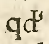
\includegraphics[height=06ex]{img/27a-1_Zaborowski_Polona03_quod}
    
\includegraphics[height=06ex]{img/27a-2_Zaborowski_Polona08_quod}
    \caption{On the left Capelli's dictionary, next Zaborowski's treatise (1518)}
    \label{fig:dzawijas}
  \end{figure}

  
\item [0xF0008] LATIN SMALL LETTER D WITH HIGH OVERLINE VARIANT:\\
  \Jglyph{󰀈}.\\ Cf. \url{https://github.com/psb1558/Junicode-New/discussions/44#discussioncomment-202860}.

    In JuniusX font accessible  with \texttt{ss04};
  cf. \autocite[p. 6]{baker20:_opent_featur_junius_junius}.

  
\item [0xF0009] LATIN CAPITAL LETTER E WITH STROKE THROUGH TERMINAL VARIANT [JuniusX]:\\
  \Jglyph{󰀉}.\\ Cf. \url{https://github.com/psb1558/Junicode-New/issues/13}.
  
  In JuniusX font accessible also as \textit{Ę} with \texttt{cv08[2]};
  cf. \autocite[p. 8]{baker20:_opent_featur_junius_junius}.

 May be considered also as a variant of LATIN CAPITAL LETTER E WITH
 STROKE (U+0246).

 Occurs in particular in \textit{Nowe Ateny} (Supplement 1774,
 \url{http://www.wbc.poznan.pl/Content/6663/index.djvu?djvuopts=&page=1783.djvu},
 cf. Fig. \vref{fig:NA1774}.
 

  \begin{figure}[h]
    
\includegraphics[width=1.3\textwidth]{img/00435077wezach}
    \caption{\J W󰀉ZACH (1774)}
    \label{fig:NA1774}
  \end{figure}

 \item [0xF000A] LATIN SMALL LETTER E WITH STROKE THROUGH TERMINAL VARIANT [JuniusX]:\\
  \Jglyph{󰀊}.\\ Cf. \url{https://github.com/psb1558/Junicode-New/issues/13}.

  In JuniusX font accessible also as \textit{ę} with \texttt{cv08[2]};
  cf. \autocite[p. 7]{baker20:_opent_featur_junius_junius}.

  For completeness it should be noted that there is also the variant
  \texttt{cv08[1]} of \textit{ę} intended for the Latin abbreviation
  of \textit{AE}.

 Occurs in particular in \textit{List o oblężeniu zamku Dyjamenckiego} (1605,
 \url{https://cbdu.ijp.pan.pl/id/eprint/2910/},
 cf. Fig. \vref{fig:e1605}.
 
  \begin{figure}[h]
    
\includegraphics[width=1\hsize]{img/00436649jezyk}
    \caption{\J j󰀊zyk (1605)}
    \label{fig:e1605}
  \end{figure}

 May be considered also as a variant of LATIN SMALL LETTER E WITH
  STROKE (U+0247).

\item [0xF000B] LATIN SMALL LETTER F CONTEXTUAL VARIANT [JuniusX]:\\
  \Jglyph{󰀋}.\\ Used e.g. before vowels with dieresis,
  cf. \url{https://github.com/psb1558/Junicode-New/discussions/44#discussioncomment-208296}.
  
  In JuniusX font accessible also as \textit{f} with \texttt{cv09[5]};
  cf. \autocite[p. 9]{baker20:_opent_featur_junius_junius}, and used
  in proper contexts by \texttt{calt} (Contextual Alternates).
  
\item [0xF000C] LATIN SMALL LETTER I WITH HIGH OVERLINE VARIANT [JuniusX]:\\
  \Jglyph{󰀌}.\\ Cf. \url{https://github.com/psb1558/Junicode-New/discussions/44#discussioncomment-202860}.

  In JuniusX font accessible  with \texttt{ss04};
  cf. \autocite[p. 6]{baker20:_opent_featur_junius_junius}.

\item [0xF000D] LATIN SMALL LETTER J CONTEXTUAL VARIANT [JuniusX]:\\
  \Jglyph{󰀍}.\\ Used when the letter is preceded by g or certain vowels with ogonek,
  cf. \url{https://github.com/psb1558/Junicode-New/discussions/44#discussioncomment-208296}.

  % In JuniusX font accessible also as \textit{đ}  (U+0111) with \texttt{cv06[1]};
  % cf. \autocite[p. 7]{baker20:_opent_featur_junius_junius}.
  In JuniusX font used
  in proper contexts by \texttt{calt} (Contextual Alternates).

\item [0xF000E] LATIN SMALL LETTER J WITH HIGH OVERLINE VARIANT [JuniusX]:\\
  \Jglyph{󰀎}.\\ Cf. \url{https://github.com/psb1558/Junicode-New/discussions/44#discussioncomment-202860}.

  In JuniusX font accessible  with \texttt{ss04};
  cf. \autocite[p. 6]{baker20:_opent_featur_junius_junius}.

\item [0xF000F] LATIN SMALL LETTER L WITH HIGH ROUNDED STROKE VARIANT [JuniusX]:\\
  \Jglyph{󰀏}.\\  Cf. \url{https://github.com/psb1558/Junicode-New/issues/4}.

  In JuniusX font accessible also as
  % textit
  ꝉ
  (LATIN SMALL LETTER L WITH HIGH STROKE,
 U+A749) with \texttt{cv17[1]};
  cf. \autocite[p. 9]{baker20:_opent_featur_junius_junius}.

  Used in Latin as an abbreviation, cf. \autocite{balbi1460:_cathol},
  quoted after \autocite[s. 6]{N3027}. 
  
  The character occurs in particular in Zaborowski's treatise as the
  abbreviation, cf. \vref{fig:l}, but also in the function of the
  present day \textit{ł}.

  \begin{figure}[h]
    \centering
    \includegraphics[height=06ex]{img/23-1_Zaborowski_WBC_9_vel}
    \includegraphics[height=06ex]{img/23-2_Zaborowski_Polona_7_vel}
    \includegraphics[height=06ex]{img/23-3_Zaborowski_WBC_4_regula}
    \includegraphics[height=06ex]{img/23-4_Zaborowski_Polona_7_populus}
    \caption{From the left: \textit{vel} (1514-1515) and 1518), \textit{regula} (1514-1515), \textit{populus} (1518)}
    \label{fig:l}
  \end{figure}
  
\item [0xF0010] LATIN SMALL LETTER M WITH HIGH OVERLINE VARIANT [JuniusX]:\\
  \Jglyph{󰀐}.\\ Cf. \url{https://github.com/psb1558/Junicode-New/discussions/44#discussioncomment-202860}.

  In JuniusX font accessible  with \texttt{ss04};
  cf. \autocite[p. 6]{baker20:_opent_featur_junius_junius}.

 \item [0xF0011] LATIN SMALL LETTER O WITH STROKE HORNED VARIANT [JuniusX]\\
  \Jglyph{󰀑}.\\  Cf. \url{https://github.com/psb1558/Junicode-New/issues/3}.
  In JuniusX font accessible also as \textit{ø} (U+00F8) with \texttt{cv21[1]};
  cf. \autocite[p. 9]{baker20:_opent_featur_junius_junius}.

  % \cite{al.55:_zasad}
  The principles of editing old Polish texts
  \autocite{Górski_Konrad__Zasady} mention the character, but don't
  give specific examples. Nevertheless they recommend to use it in
  critical editions.
  
\item [0xF0012] LATIN SMALL LETTER O WITH SHIFTED STROKE VARIANT [JuniusX]\\:
  \Jglyph{󰀒}.\\  Cf. \url{https://github.com/psb1558/Junicode-New/issues/3}.
  
  In JuniusX font accessible also as \textit{ø} (U+00F8) with \texttt{cv21[2]};
 cf. \autocite[p. 9]{baker20:_opent_featur_junius_junius}.

 The principles of editing old Polish texts
  \autocite{Górski_Konrad__Zasady} mention the character, but don't
  give specific examples. 

\item [0xF0013] LATIN SMALL LETTER O WITH STROKE HORN DOWNWARDS VARIANT [JuniusX]\\:
  \Jglyph{󰀓}.\\  Cf. \url{https://github.com/psb1558/Junicode-New/issues/3}.

  In JuniusX font accessible also as \textit{ø} (U+00F8) with \texttt{cv21[3]};
  cf. \autocite[p. 9]{baker20:_opent_featur_junius_junius}.

 The principles of editing old Polish texts
  \autocite{Górski_Konrad__Zasady} mention the character, but don't
  give specific examples. 


\item [0xF0014] LATIN SMALL LETTER O WITH STROKE HORN UPWARDS VARIANT [JuniusX]\\:
  \Jglyph{󰀓}.\\  Cf. \url{https://github.com/psb1558/Junicode-New/issues/3}.

  In JuniusX font accessible also as \textit{ø} (U+00F8) with \texttt{cv21[4]};
  cf. \autocite[p. 9]{baker20:_opent_featur_junius_junius}.

 The principles of editing old Polish texts
  \autocite{Górski_Konrad__Zasady} mention the character, but don't
  give specific examples. 



\item [0xF0015] MEDIEVAL SUPERSCRIPT LETTER Q [JuniusX]\\:
  \Jglyph{󰀕}.\\
  Cf. \url{https://github.com/psb1558/Junicode-New/discussions/44#discussioncomment-208296}.

  In JuniusX font accessible also as \texttt{sup} (Superscripts).

  % q

\item [0xF0016] LATIN SMALL LETTER RUM ROTUNDA VARIANT [JuniusX]\\:
  \Jglyph{󰀖}.\\%  Cf. \url{https://github.com/psb1558/Junicode-New/issues/3}.

  In JuniusX font accessible also as \textit{ꝝ} (U+A75D) with \texttt{cv41[1]};
  cf. \autocite[p. 12]{baker20:_opent_featur_junius_junius}.
\item [0xF0017] LATIN SMALL LETTER V WITH MEDIUM HIGH OVERLINE VARIANT [JuniusX]:\\
  \Jglyph{󰀗}.\\ Cf. \url{https://github.com/psb1558/Junicode-New/discussions/44#discussioncomment-202860}.

      In JuniusX font accessible  with \texttt{ss05};
  cf. \autocite[p. 7]{baker20:_opent_featur_junius_junius}.

  
\item [0xF0018] LATIN SMALL LETTER V WITH HIGH OVERLINE VARIANT [JuniusX]:// 
  \Jglyph{󰀘}.\\ Cf. \url{https://github.com/psb1558/Junicode-New/discussions/44#discussioncomment-202860}.

  In JuniusX font accessible  with \texttt{ss04};
  cf. \autocite[p. 6]{baker20:_opent_featur_junius_junius}.


\item [0xF0019] LATIN SMALL LETTER X WITH MEDIUM HIGH OVERLINE VARIANT [JuniusX]:// 
  \Jglyph{󰀙}.\\ Cf. \url{https://github.com/psb1558/Junicode-New/discussions/44#discussioncomment-202860}.

  
      In JuniusX font accessible  with \texttt{ss05};
  cf. \autocite[p. 7]{baker20:_opent_featur_junius_junius}.

% x
\item [0xF001A] LATIN SMALL LETTER X WITH HIGH OVERLINE VARIANT [JuniusX]:// 
  \Jglyph{󰀚}.\\ Cf. \url{https://github.com/psb1558/Junicode-New/discussions/44#discussioncomment-202860}.

    In JuniusX font accessible  with \texttt{ss04};
  cf. \autocite[p. 6]{baker20:_opent_featur_junius_junius}.


\item [0xF001B] LATIN LETTER GLOTTAL STOP VARIANT [JuniusX]\\
  \Jglyph{󰀛}.\\%  Cf. \url{https://github.com/psb1558/Junicode-New/issues/??}.
% \\item [0xF001C] LATIN SMALL LETTER RUM ROTUNDA VARIANT [JuniusX]\\:

    In JuniusX font accessible as ʔ (U+0294)  with \texttt{cv50[1]};
  cf. \autocite[p. 11]{baker20:_opent_featur_junius_junius}.


\item [0xF001C] TIRONIAN SIGN CAPITAL ET VARIANT [JuniusX]\\:
\Jglyph{󰀜}.%\\%  Cf. \url{https://github.com/psb1558/Junicode-New/issues/??}.

In JuniusX font accessible also as \textit{⹒} (U+2E52) with \texttt{cv40[1]};
  cf. \autocite[p. 12]{baker20:_opent_featur_junius_junius}.

\item [0xF001D] TIRONIAN SIGN ET VARIANT [JuniusX]\\:
  \Jglyph{󰀝}.\\%  Cf. \url{https://github.com/psb1558/Junicode-New/issues/??}.

  In JuniusX font accessible also as \textit{⁊} (U+204A) with \texttt{cv40[1]};
  cf. \autocite[p. 12]{baker20:_opent_featur_junius_junius}.

\item[0xF001E] LATIN CAPITAL LETTER A WITH STROKE
  VARIANT [JuniusX]: \Jglyph{󰀞}.\\
  Cf. \url{https://github.com/psb1558/Junicode-New/issues/14}.
  % The
  % term \textit{terminal} used after ???.\\
  
  In JuniusX font accessible also as \textit{A} with \texttt{cv02[2]};
  cf. \autocite[p. 7]{baker20:_opent_featur_junius_junius}.
% 
%  Used in particular in ???, cf. Fig. ???

    May be considered also as a variant of LATIN CAPITAL LETTER A WITH
  STROKE (U+023A).

  
\item [0xF001F] LATIN SMALL LETTER A WITH STROKE  VARIANT [JuniusX]: 
  \Jglyph{󰀟}.\\ Cf. \url{https://github.com/psb1558/Junicode-New/issues/14}.
  % The
  % term \textit{terminal} used after ???.

  In JuniusX font accessible also as \textit{A} with \texttt{cv02[2]};
  cf. \autocite[p. 7]{baker20:_opent_featur_junius_junius}.

  May be considered also as a variant of LATIN SMALL LETTER A WITH
  STROKE (U+2C65).
\item[dolne]
  Kazania świętokrzyskie
s.12 kazanie III na dzięń św. Mikołaja

Sankt Florian Psalter Holy Cross Sermons

  \cite{vrtel-wierczyński50:_wybór} photo-offset

\end{description}

\autocite{wydra14:_oldes_extan_prose_text_polis}

Repository!!!
\printbibliography
\end{document}

– Nowe Ateny albo Akademia wszelkiey scyencyi pełna,
na różne tytuły iak na classes podzielona, mądrym
dla memoryału, idiotom dla nauki, politykom dla
praktyki, melancholikom dla rozrywki erygowana ...
/ przez Xiędza Benedykta Chmielowskiego ...
.
Część 1.2. http://www.wbc.poznan.pl/publication/3735,
publication date 1756??? (drugie wydanie), 844 pages.

Nowe Ateny, albo Akademia wszelkiey scyencyi pełna, na różne tytuły
iak na classes podzielona, mądrym dla memoryału, idiotom dla nauki,
politykom dla praktyki, melancholikom dla rozrywki erygowana
... . Część 3 albo Supplement.
Nowe Ateny, albo Akademia wszelkiey scyencyi pełna,
na różne tytuły iak na classes podzielona, mądrym
dla memoryału, idiotom dla nauki, politykom dla
praktyki, melancholikom dla rozrywki erygowana ...
. Część 3 albo Supplement.. http://www.wbc.poznan.
pl/publication/37543, publication date 1754, 741 pages.


DżZ. Zbiór rytmów duchownych Panegirycznych Moral- nych i
Swiatowych [...] Elżbiety z Kowalskich Druzback- iey [...] Zebrany y
do druku podany przez J. Z. R. K.  O. W. etc. [Załuskiego Józefa
Andrzeja]. http://www.wbc.poznan.pl/publication/13950, publication
date 1752, 566 pages.

List o oblężeniu zamku Dyjamenckiego w Inflantach do Krzysztofa Moniwida Dorohostajskiego, dnia 22 października 1605 pisany

http://cbdu.id.uw.edu.pl/2910/1/Z291.djvu?djvuopts=&page=0006l.djvu 

https://cbdu.ijp.pan.pl/id/eprint/2910/

ä

%%% Local Variables: 
%%% coding: utf-8-unix
%%% eval: (set-fontset-font "fontset-default" '(#xF0000 . #xF001F) (font-spec :size 18 :name "JuniusX"))
%%% mode: latex
%%% TeX-master: t
%%% TeX-PDF-mode: t
%%% TeX-engine: xetex
%%% End: 
